\documentclass[border=6pt,tikz]{standalone}
\usepackage{tikz}
\usepackage{amsmath,amssymb}
\usetikzlibrary{arrows.meta,positioning,fit,backgrounds,calc,shapes.geometric,decorations.pathreplacing,patterns}
\definecolor{ink}{HTML}{1B2430}
\definecolor{muted}{HTML}{6B7785}
\definecolor{accent}{HTML}{2F6FB5}
\definecolor{accent2}{HTML}{C1611F}
\definecolor{good}{HTML}{2E7D5B}
\definecolor{soft}{HTML}{EDF2F7}
\definecolor{soft2}{HTML}{FBEDE2}
\definecolor{soft3}{HTML}{E6F0E9}
\tikzset{
  box/.style={draw=ink,line width=.7pt,rounded corners=2pt,fill=soft,inner sep=4pt,align=center,font=\sffamily\small},
  boxa/.style={box,fill=soft2},
  boxb/.style={box,fill=soft3},
  plain/.style={align=center,font=\sffamily\small,text=ink},
  tiny/.style={align=center,font=\sffamily\scriptsize,text=muted},
  ar/.style={-{Stealth[length=2.4mm]},draw=ink,line width=.7pt},
  arm/.style={-{Stealth[length=2.4mm]},draw=muted,line width=.6pt,dashed},
  nd/.style={circle,draw=ink,line width=.7pt,fill=white,minimum size=7mm,inner sep=0pt,font=\sffamily\scriptsize},
  ndf/.style={nd,fill=soft},
  ndt/.style={nd,fill=soft2},
}

\begin{document}

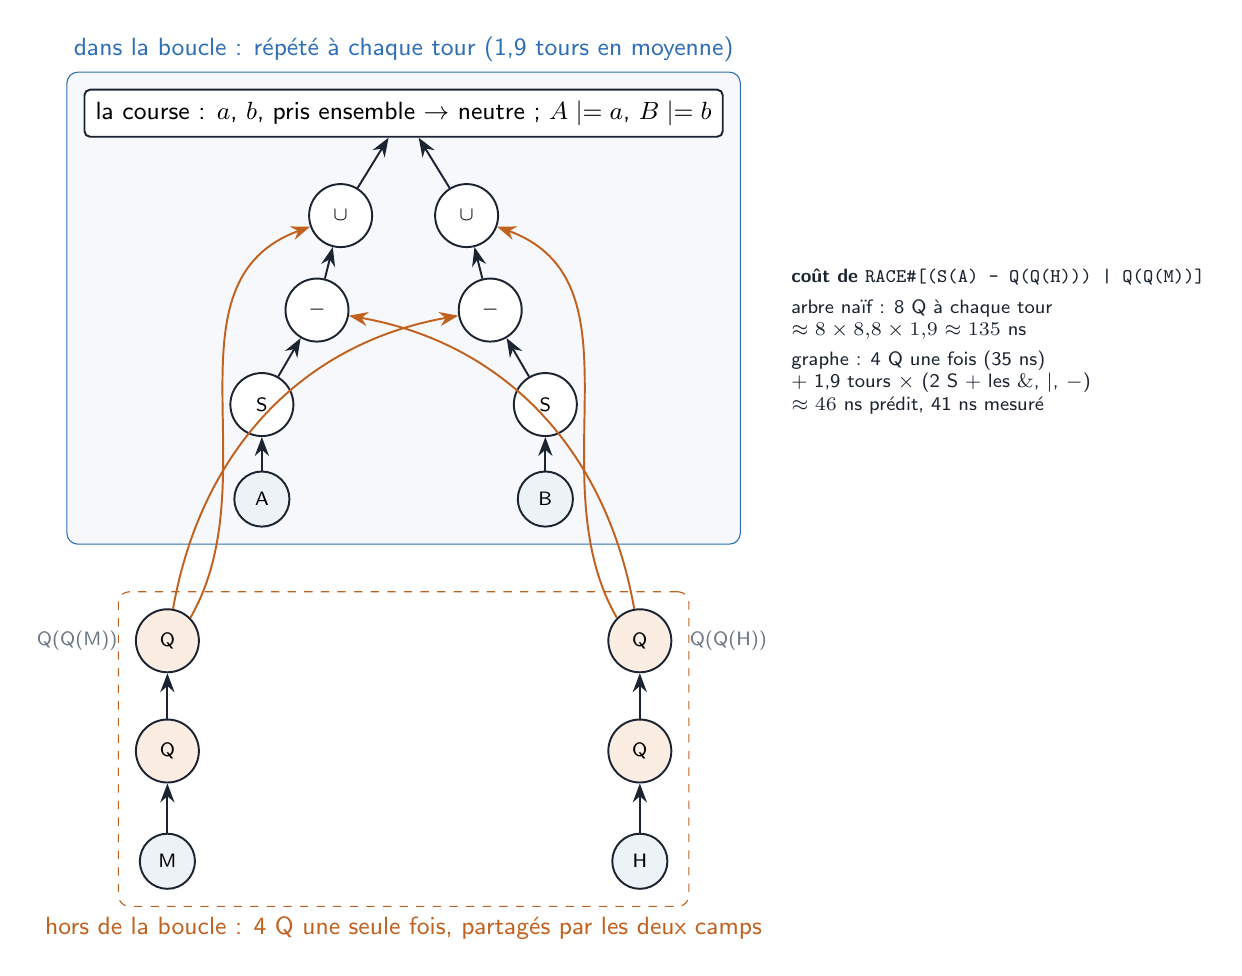
\begin{tikzpicture}[x=1cm,y=1cm,
  op/.style={nd,minimum size=8mm},
  q/.style={nd,fill=soft2,minimum size=8mm},
  lf/.style={nd,fill=soft,minimum size=7mm}]
% leaves and hoisted part
\node[lf] (M) at (0,0) {M};
\node[lf] (H) at (6,0) {H};
\node[q] (QM) at (0,1.4) {Q};
\node[q] (QH) at (6,1.4) {Q};
\node[q] (QQM) at (0,2.8) {Q};
\node[q] (QQH) at (6,2.8) {Q};
\node[tiny,left=1mm of QQM] {Q(Q(M))};
\node[tiny,right=1mm of QQH] {Q(Q(H))};
\draw[ar] (M) -- (QM); \draw[ar] (QM) -- (QQM);
\draw[ar] (H) -- (QH); \draw[ar] (QH) -- (QQH);
\begin{scope}[on background layer]
\node[draw=accent2,dashed,rounded corners,fit=(M)(QQM)(H)(QQH),inner sep=6pt,
  label={[plain,text=accent2]below:hors de la boucle : 4 Q une seule fois, partagés par les deux camps}] {};
\end{scope}
% loop body
\node[lf] (A) at (1.2,4.6) {A};
\node[op] (SA) at (1.2,5.8) {S};
\node[op] (mA) at (1.9,7.0) {$-$};
\node[op] (oA) at (2.2,8.2) {$\cup$};
\node[lf] (B) at (4.8,4.6) {B};
\node[op] (SB) at (4.8,5.8) {S};
\node[op] (mB) at (4.1,7.0) {$-$};
\node[op] (oB) at (3.8,8.2) {$\cup$};
\draw[ar] (A) -- (SA); \draw[ar] (SA) -- (mA); \draw[ar] (mA) -- (oA);
\draw[ar] (B) -- (SB); \draw[ar] (SB) -- (mB); \draw[ar] (mB) -- (oB);
\draw[ar,accent2] (QQH) to[out=100,in=-10] (mA);
\draw[ar,accent2] (QQM) to[out=80,in=190] (mB);
\draw[ar,accent2] (QQM.north east) to[out=60,in=200] (oA);
\draw[ar,accent2] (QQH.north west) to[out=120,in=-20] (oB);
\node[box,fill=white] (race) at (3,9.5) {la course : $a$, $b$, pris ensemble $\to$ neutre ; $A \mathrel{|}= a$, $B \mathrel{|}= b$};
\draw[ar] (oA) -- (race); \draw[ar] (oB) -- (race);
\begin{scope}[on background layer]
\node[draw=accent,rounded corners,fill=soft!50,fit=(A)(B)(race),inner sep=6pt,
  label={[plain,text=accent,align=center]above:dans la boucle : répété à chaque tour (1,9 tours en moyenne)}] {};
\end{scope}
\node[tiny,text=ink,align=left,anchor=west] at (7.8,6.6) {\textbf{coût de \texttt{RACE\#[(S(A) - Q(Q(H))) | Q(Q(M))]}}\\[3pt]
arbre naïf : 8 Q à chaque tour\\$\approx 8 \times 8{,}8 \times 1{,}9 \approx 135$ ns\\[3pt]
graphe : 4 Q une fois (35 ns)\\+ 1,9 tours $\times$ (2 S + les $\&$, $|$, $-$)\\$\approx 46$ ns prédit, 41 ns mesuré};
\end{tikzpicture}
\end{document}
